\subsection{Build RAVEN input: \xmlNode{SingleRun}}
In this section, we will show the user how to use RAVEN to run a single instance of a driven code, plotting and
printing some variables.. 
\subsubsection{Set up a simple RAVEN input}
We will start to build a very simple RAVEN input. From this process, we hope the user can get a better idea about
RAVEN \textbf{Entities} and learn how to build their own RAVEN inputs for their applications.
In order to accomplish these tasks, the following steps are needed:
\begin{enumerate}
   \item \textbf{Set up the running environment}: \xmlNode{RunInfo}
   \item \textbf{Provide the required files}: \xmlNode{Files}
   \item \textbf{Link between RAVEN and driven code}: \xmlNode{Models}
   \item \textbf{Container of input and output data}: \xmlNode{DataObjects}
   \item \textbf{Control of executions}: \xmlNode{Steps}
\end{enumerate}
The RAVEN input file will look like:
\xmlExample{framework/user_guide/SingleRuns/singleRun.xml}{Simulation}
In this specific case, as shown in \xmlNode{RunInfo}, only one step named \xmlString{singleRun} is going to be
sequentially run using a single processor as defined by \xmlNode{BatchSize}. All the output files and temporary
files will be dumped in the folder \xmlString{singleRunAnalysis}.The \xmlNode{Steps} will be used to
link the rest of \textbf{Entities} to perform a single run, i.e. load the input file \xmlString{referenceInput.xml} as defined in
\xmlNode{Files} via \xmlNode{Input}, run the code using the commands defined in \xmlNode{Models}, and collect the
input and output data into the data objects \xmlString{history} which is defined as \xmlNode{HistorySet} to store
the time-dependent data..
The subnodes defined for \xmlNode{Code} is equivalent to:
\begin{lstlisting}[language=bash]
python ../physicalCode/analyticalbateman/AnalyticalDplMain.py
\end{lstlisting}
with the requirement of extensions of input and output files, as defined via \xmlNode{clargs}, to be \xmlString{.xml} and \xmlString{.csv},
respectively.
In addition, the \xmlString{GenericCode} interface is used for this case since the driven code already dumps its
outputs in CSV format. In general, the users need to create an ad-hoc code interface for their applications. More
detailed information can be found in ~\cite{RAVENuserManual}. 

\subsubsection{Output: print and plot using \xmlNode{OutStreams}}
\xmlNode{OutStreams} can be used to visualize and dump out the data that is generated, imported or post-processed during
the analysis. It supports two actions:
\begin{enumerate}
  \item \textbf{Print}: module that lets the user dump the data contained in the internal objects;
  \item \textbf{Plot}: module based on MatPLotLib~\cite{MatPlotLib}, aimed to provide advanced plotting capabilities.
\end{enumerate}
Both actions listed above accept a \xmlString{DataObject} as an \xmlNode{Input}. The printing system has been created
in order to let he user dump the data, contained in the internal data objects, out at anytime during the calculation.
The plotting system provides all the capabilities to visualize the analysis outcomes, in real-time or as a post-processing
stage.

\begin{enumerate}
   \item \textbf{\textit{OutStreams}}:
     \xmlExample{framework/user_guide/SingleRuns/singleRunPlotAndPrint.xml}{OutStreams}
  In this block, both the Out-Stream types are constructed:
  \begin{itemize}
    \item \textit{Print}:
     \begin{itemize}
       \item named "pointValues" connected with the \textit{DataObjects} \textbf{Entity} ``pointValues'' (\xmlNode{source})
       \item named ``history'' connected with the \textit{DataObjects} \textbf{Entity} ``history'' (\xmlNode{source})
     \end{itemize}
      When this objects get used, all the information contained in the linked  \textit{DataObjects} are going
    to be dumped in CSV files (\xmlNode{type}).
    \item \textit{Plot}: a single \xmlNode{Plot} \textbf{Entity} is defined, containing the line plots of the 4 output variables
    ($A,B,C,D$) in the same figure. This object is going to generate a PNG file and an interactive Plot on
    the screen.
  \end{itemize}
 %%%%%%%%%%%%%%%%%%%%%%%%%%%%%%%%%%%%%%%%%%%%%%%%%%%%%%%%%%
 %figure history
 \begin{figure}[h!]
  \centering
  \includegraphics[scale=0.7]{../../tests/framework/user_guide/SingleRuns/gold/singleRunPlot/1-historyPlot_line-line-line-line.png}
  \caption{Plot of the history for variables $A,B,C,D$.}
  \label{fig:historyPlotLine}
 \end{figure}
 %%%%%%%%%%%%%%%%%%%%%%%%%%%%%%%%%%%%%%%%%%%%%%%%%%%%%%%%%%
\end{enumerate}

\subsubsection{IOStep: perform input/output operations}
The \xmlNode{IOStep} acts as a "transfer network" among different RAVEN storing or streaming objects. The number
of \xmlNode{Input} and \xmlNode{Output} is unlimited. This \xmlNode{IOStep} assumes one-to-one maping, i.e. the first
\xmlNode{Input} is going to be used for the first \xmlNode{Output}, etc. \nb If the \xmlNode{Output} nodes are class
\xmlString{OutStreams}, the user does not need to follow this assumption, since \textbf{OutStreams} objects are already
lined to \textbf{DataObjects} in the relative RAVEN input block.

\begin{enumerate}
   \item \textbf{\textit{IOStep}}:
     \xmlExample{framework/user_guide/SingleRuns/singleRunPlotAndPrint.xml}{Steps}
\end{enumerate}

For examples of the numerical data produced by the OutStreams \textit{Print}, see \texttt{history\_0.csv} in the directory
 \texttt{raven/tests/framework/user\_guide/SingleRuns/gold/singleRunPlot/}
 As previously mentioned, Figure~\ref{fig:historyPlotLine} reports the four plots (four variables) drawn in the same picture.

%\FloatBarrier
\subsubsection{OutStream System: Sub-plot and Selectively print.}
This Section shows how to use RAVEN to create sub-plots (multiple plots in the same figure) and
how to select only some variable from the \textit{DataObjects} in the \textit{Print} OutStream.
 \\ The goals of this Section are about learning how to:
 \begin{enumerate}
   \item Print out what contained in the DataObjects, selecting only few variables
   \item Generate sub-plots (multiple plots in the same figure) of the code results
\end{enumerate}

To accomplish these tasks, the \textit{OutStreams} \textbf{Entity} in the input defined in the previous section needs to be modified as follows:
\xmlExample{framework/user_guide/SingleRuns/singleRunSubPlotsAndSelectivePrint.xml}{OutStreams}
\begin{enumerate}
   \item \textbf{\textit{Print}}:
   With respect to the \textit{Print} nodes defined in the previous section, it can
   be noticed that an additional node has been added: \xmlNode{what}. The \textit{Print} \textbf{Entity}
   ``pointValues'' is going to extract and dump only the variables that are part of the Output space
   ($A,B,C,D$ and not $InputPlaceHolder$).  The \textit{Print} \textbf{Entity} ``history'' is instead going to print
   the Output space variables $A$ and $D$.

   \item \textbf{\textit{Plot}}:
 Note that the  \textit{Plot} \textbf{Entity} does not differ much with respect to the one in
 previous section: 1) the additional sub-node \xmlNode{gridSpace}  has been added.
 This node is needed to define how the figure needs to be partitioned (discretization of the grid). In this case
 a 2 by 2 grid is requested. 2) in each \xmlNode{plot} the node \xmlNode{gridLocation} is placed in
 order to specify in which position the relative plot needs to be placed. For example, in the following grid
 location, the relative plot is going to be placed at the bottom-right corner.
  \begin{lstlisting}[style=XML,morekeywords={arg,extension,pauseAtEnd,overwrite}]
   <gridLocation>
      <x>1</x>
      <y>1</y>
   </gridLocation>
   \end{lstlisting}
 \end{enumerate}
The CSV tables generated by the \textit{Print} \textbf{Entities} are not reported, since the only differences with respect to Tables ~\ref{historyVI.I} and ~\ref{pointValuesVI.I} are related to the number of columns (variables)
dumped out.
\\Figure~\ref{fig:historySubPlotLine} reports the four plots (four variables) drawn in the same picture.
 %figure history sublots
 \begin{figure}[h!]
  \centering
  \includegraphics[scale=0.7]{../../tests/framework/user_guide/SingleRuns/gold/subPlot/1-historyPlot_line-line-line-line.png}
  \caption{Subplot of the history for variables $A,B,C,D$.}
  \label{fig:historySubPlotLine}
 \end{figure}

